% !TeX spellcheck = sl_SI
% vim: set spell spelllang=sl:
% za preverjanje črkovanja, če se uporablja Texstudio ali vim
\documentclass[12pt,a4paper,twoside]{article}
\usepackage[utf8]{inputenc}  % pravilno razpoznavanje unicode znakov

% NASLEDNJE UKAZE USTREZNO POPRAVI
\newcommand{\program}{Matematika} % ime studijskega programa
\newcommand{\imeavtorja}{Janez~Radešček} % ime avtorja
\newcommand{\imementorja}{doc.~dr.~Pretnar Matija} % akademski naziv in ime mentorja, uporabi poln naziv, prof.~dr.~, doc.~dr., ali izr.~prof.~dr.
\newcommand{\imesomentorja}{} % akademski naziv in ime somentorja, če ga imate
\newcommand{\naslovdela}{Naslov vašega dela}
\newcommand{\letnica}{2021} % letnica magistriranja
\newcommand{\opis}{Delo obravnava integracijo po ω-kompleksih, njene lastnosti in posplošitve
na Levy-jeve topološke prostore.}  % Opis dela v eni povedi. Ne sme vsebovati matematičnih simbolov v $ $.
\newcommand{\kljucnebesede}{integracija\sep kompleks} % ključne besede, ločene z \sep, da se PDF metapodatki prav procesirajo
\newcommand{\keywords}{integration\sep complex} % ključne besede v angleščini
\newcommand{\organization}{Univerza v Ljubljani, Fakulteta za matematiko in fiziko} % fakulteta
\newcommand{\literatura}{literatura}  % pot do datoteke z literaturo (brez .bib končnice)
\newcommand{\sep}{, }  % separator med ključnimi besedami v besedilu
% KONEC PODATKOV

\usepackage{bibentry}         % za navajanje literature v programu dela s celim imenom
\nobibliography{\literatura}
\newcommand{\plancite}[1]{\item[\cite{#1}] \bibentry{#1}} % citiranje v programu dela

\usepackage{filecontents}  % za pisanje datoteke s PDF metapodatki
\usepackage{silence} \WarningFilter{latex}{Overwriting file}  % odstrani annoying warning o obstoju datoteke
% datoteka s PDF metapodatki, zgenerira se kot magisterij.xmpdata
\begin{filecontents*}{\jobname.xmpdata}
  \Title{\naslovdela}
  \Author{\imeavtorja}
  \Keywords{\kljucnebesede}
  \Subject{matematika}
  \Org{\organization}
\end{filecontents*}

\usepackage[a-1b]{pdfx}  % zgenerira PDF v tem PDF/A-1b formatu, kot zahteva knjižnica
\hypersetup{bookmarksopen, bookmarksdepth=3, colorlinks=true,
  linkcolor=black, anchorcolor=black, citecolor=black, filecolor=black,
  menucolor=black, runcolor=black, urlcolor=black, pdfencoding=auto,
  breaklinks=true, psdextra}

\usepackage[slovene]{babel}  % slovenščina
\usepackage[T1]{fontenc}     % naprednejše kodiranje fonta
\usepackage{amsmath,amssymb,amsfonts,amsthm} % matematični paketi
\usepackage{graphicx}     % za slike
\usepackage{emptypage}    % prazne strani so neoštevilčene, ampak so štete
\usepackage{units}        % fizikalne enote kot \unit[12]{kg} s polovico nedeljivega presledka, glej primer v kodi
\usepackage{makeidx}      % za stvarno kazalo, lahko zakomentiraš, če ne rabiš
\makeindex                % za stvarno kazalo, lahko zakomentiraš, če ne rabiš
% oblika strani
\usepackage[
  top=3cm,
  bottom=3cm,
  inner=3.5cm,      % margini za dvostransko tiskanje
  outer=2.5cm,
  footskip=40pt     % pozicija številke strani
]{geometry}

% VEČ ZANIMIVIH PAKETOV
% \usepackage{array}      % več možnosti za tabele
% \usepackage[list=true,listformat=simple]{subcaption}  % več kot ena slika na figure, omogoči slika 1a, slika 1b
% \usepackage[all]{xy}    % diagrami
% \usepackage{doi}        % za clickable DOI entrye v bibliografiji
% \usepackage{enumerate}     % več možnosti za sezname

% Za barvanje source kode
\usepackage{minted}
\renewcommand\listingscaption{Program}

% Za pisanje psevdokode
% \usepackage{algpseudocode}  % za psevdokodo
% \usepackage{algorithm}
% \floatname{algorithm}{Algoritem}
% \renewcommand{\listalgorithmname}{Kazalo algoritmov}

% DRUGI TVOJI PAKETI:
% tukaj
\usepackage{listings}

%\usepackage[dvipsnames]{xcolor}

\definecolor{jcyan}{cmyk}{1, 0, 0.15, 0.05}
\definecolor{jyellow}{cmyk}{0.8, 0, 0.4, 0}
% todo notes to comment the code when working in a group
\usepackage{todonotes}
\newcommand\dic[1]{\todo[inline,color=yellow]{#1}}	% slovar
\newcommand\mP[1]{\todo[inline,color=red]{#1 -MP}}	% comments by matija
\newcommand\jR[1]{\todo[inline,color=jcyan]{#1 -JR}} % comments by janez

%

\setlength{\overfullrule}{50pt} % označi predlogo vrstico
\pagestyle{plain}               % samo številka strani na dnu, nobene glave / noge

% ukazi za matematična okolja
\theoremstyle{definition} % tekst napisan pokončno
\newtheorem{definicija}{Definicija}[section]
\newtheorem{primer}[definicija]{Primer}
\newtheorem{opomba}[definicija]{Opomba}
\newtheorem{aksiom}{Aksiom}

\theoremstyle{plain} % tekst napisan poševno
\newtheorem{lema}[definicija]{Lema}
\newtheorem{izrek}[definicija]{Izrek}
\newtheorem{trditev}[definicija]{Trditev}
\newtheorem{posledica}[definicija]{Posledica}

\numberwithin{equation}{section}  % števec za enačbe zgleda kot (2.7) in se resetira v vsakem poglavju

% Matematični ukazi
\newcommand{\R}{\mathbb R}
\newcommand{\N}{\mathbb N}
\newcommand{\Z}{\mathbb Z}
\newcommand{\C}{\mathbb C}
\newcommand{\Q}{\mathbb Q}

\newcommand{\lae}{$\lambda_{\text{\ae}}$} % the name of the calculus
\newcommand{\aeff}{Æff} % the name of the language

% \DeclareMathOperator{\tr}{tr}  % morda potrebuješ operator za sled ali kaj drugega?

% bold matematika znotraj \textbf{ }, tudi v naslovih, kot \omega spodaj
\makeatletter \g@addto@macro\bfseries{\boldmath} \makeatother

% Poimenuj kazalo slik kot ``Kazalo slik'' in ne ``Slike''
\addto\captionsslovene{
  \renewcommand{\listfigurename}{Kazalo slik}%
}

% če želiš, da se poglavja začnejo na lihih straneh zgoraj
% \let\oldsection\section
% \def\section{\cleardoublepage\oldsection}

%%%%%%%%%%%%%%%%%%%%%%%%%%%%%%%%%%%%%%%%%%
%%%%%%           DOCUMENT           %%%%%%
%%%%%%%%%%%%%%%%%%%%%%%%%%%%%%%%%%%%%%%%%%

\begin{document}

\pagenumbering{roman} % začnemo z rimskimi številkami
\thispagestyle{empty} % ampak na prvi strani ni številke

\noindent{\large
UNIVERZA V LJUBLJANI\\[1mm]
FAKULTETA ZA MATEMATIKO IN FIZIKO\\[5mm]
\program\ -- 2.~stopnja}
% ustrezno dopolni za IŠRM
\vfill

\begin{center}
  \large
  \imeavtorja\\[3mm]
  \Large
  \textbf{\MakeUppercase{\naslovdela}}\\[10mm]
  \large
  Magistrsko delo \\[1cm]
  Mentor: \imementorja \\[2mm] % ustrezno popravi spol
%   Somentor: \imesomentorja   % dodaj, če potrebno
\end{center}
\vfill

\noindent{\large Ljubljana, \letnica}

\cleardoublepage

%% sem pride IZJAVA O AVTORSTVU  -- SE NATISNE V VIS

% zahvala
\pdfbookmark[1]{Zahvala}{zahvala} %
\section*{Zahvala}
Neobvezno.
Zahvaljujem se \dots
% end zahvala -- izbriši vse med zahvala in end zahvala, če je ne rabiš

\cleardoublepage

\pdfbookmark[1]{\contentsname}{kazalo-vsebine}
\tableofcontents

% list of figures
% \cleardoublepage
% \pdfbookmark[1]{\listfigurename}{kazalo-slik}
% \listoffigures
% end list of figures

\cleardoublepage

\section*{Program dela}
\addcontentsline{toc}{section}{Program dela} % dodajmo v kazalo
Mentor naj napiše program dela skupaj z osnovno literaturo. Na literaturo se
lahko sklicuje kot~\cite{lebedev2009introduction}, \cite{gurtin1982introduction},
\cite{zienkiewicz2000finite}, \cite{STtemplate}.

\section*{Osnovna literatura}
Literatura mora biti tukaj posebej samostojno navedena (po pomembnosti) in ne
le citirana. V tem razdelku literature ne oštevilčimo po svoje, ampak uporabljamo
okolje itemize in ukaz plancite, saj je celotna literatura oštevilčena na koncu.
\begin{itemize}
  \plancite{lebedev2009introduction}
  \plancite{gurtin1982introduction}
  \plancite{zienkiewicz2000finite}
  \plancite{STtemplate}
\end{itemize}

\vspace{2cm}
\hspace*{\fill} Podpis mentorja: \phantom{prostor za podpis}

% \vspace{2cm}
% \hspace*{\fill} Podpis somentorja: \phantom{prostor za podpis}

\cleardoublepage
\pdfbookmark[1]{Povzetek}{abstract}

\begin{center}
\textbf{\naslovdela} \\[3mm]
\textsc{Povzetek} \\[2mm]
\end{center}
%Tukaj napišemo povzetek vsebine. Sem sodi razlaga vsebine in ne opis tega, kako je delo
%organizirano.
V delu si pogledamo programski jezik \aeff\ in račun \lae\ na katerem temelji. Račun \lae razširimo z rekurzivno obljubo, razcepom in \jR{Box/Unbox}. \jR{Ground} tipe nadomestimo z mobilnimi tipi, ki nam omogočajo pošiljanje tipov za katere prej nebi zmogli pokazati da so varni. Obstoječi sistem tipov nadomestimo z dvostranskim sistemom, ki predvsem izboljša sporočila v primeru napak. Dokažemo izreka o napredku in ohranitvi za razširjen \lae. Ne deterministično operacijsko semantiko malih korakov nadomestimo z deterministično big.SMALL semantiko in pokažemo, da je prejšnji v nekem smislu ekvivalentna.



\vfill
\begin{center}
\textbf{English translation of the title} \\[3mm] % prevod slovenskega naslova dela
\textsc{Abstract}\\[2mm]
\end{center}

%An abstract of the work is written here. This includes a short description of
%the content and not the structure of your work.
TODO

\vfill\noindent
\textbf{Math.~Subj.~Class.~(2010):} oznake kot 74B05, 65N99, na voljo so na naslovu
\url{http://www.ams.org/msc/msc2010.html} \\[1mm]
\textbf{Ključne besede:} \kljucnebesede \\[1mm]
\textbf{Keywords:} \keywords

\cleardoublepage

\setcounter{page}{1}    % od sedaj naprej začni zopet z 1
\pagenumbering{arabic}  % in z arabskimi številkami


%Slovar
%promise = obljuba
%guarded promise = varovana obljuba
%abstraction = abstrakcija
%spawn = razplot? meni je lepše razcep ? 
%interpreter = interpreter
%type sistem = sistem tipov
%computation = izračun
%calculus = račun
%unit = enota
%Syntactic sugar = sintaktičen sladkor
%if computation/statement = če izračun
%parallel = vzporedno/asinhrono (Izvajamo več thredov, lahko tudi samo ne enem jedru, ampak bistveno je da vsi thredu napredujejo v nekem smislu "enakomerno". Logika program je razdeljena v več bolj ali manj neodvisnih enot threadov/procesov.)
%concurent = hkratno (dejansko izvajamo istočasno na dveh ali več jedrih), ravno obratno tu sam program morda ni napisan v večih threadih. Toda morda compiler prepozna da sta dva načeloma zaporedna izračuna neodvisna in pretvori izvorno kodo v nekaj kar zna hkrati pognati na večih jedrih.
%thread = nit
%payload = tovor
%Ground type = prizemljen/osnovni?
%mobile = mobilen
%box/boxed = okvir/okvirjen     /škatla/paket ?
%recursion = rekurzija
%bidirectional = dvostranski?
%small step semantics = op. sem. malih korakov

\jR{So zakomentirani prevodi vredu?}




\section{Uvod}
%Napišite kratek zgodovinski in matematični uvod.  Pojasnite motivacijo za problem, kje
%nastopa, kje vse je bil obravnavan. Na koncu opišite tudi organizacijo dela -- kaj je v
%katerem razdelku.

Vse pogosteje je zaželeno asinhrono izvajanje programa. 
Nekateri programski jeziki, predvsem starejše verzije, nimajo direktno podpore za asinhrono izvajanje. 
Veliko modernih jezikov, če ne drugega omogočajo tako imenovan POSIX. POSIX je API, ki na operacijskih sistemih, ki ga podpirajo, omogoča uporabo niti~\cite{posix}.
Drugi programski jeziki kot so C++, Java... imajo kot del standardne knjižnice konstrukte, ki jim omogočajo paralelno izvajanje programa. Čeprav v ozadju mnogi uporabljajo POSIX, so detajli skriti in zato bolj naravni za programerja. 
Nekateri programski jeziki omogočajo asinhono izvajanje, vendar vsaj direktno ne omogočajo hkratnega izvajanja.
Na primer CPython ima tako imenovan GIL (global  interpreter lock)~\cite{gil}, ki preprečuje interpreterju, da bi izvajal več kot eno nit na enkrat.
Le redki programski jeziki, recimo Go, pa so bili zasnovani z asinhronim programiranjem v mislih in imajo zato konstrukte potrebne za paralelno izvajanje vgrajene v jezik.

Eden izmed njih je jezik \aeff, ki sloni na računu imenovanem \lae~\cite{aeff}. \aeff je interpretiran funkcijski jezik. Glavni namen \lae je pokazati, da je v ozadju asinhronih programskih jezikov lepa teorija.

Najprej si bomo v poglavju številka \ref{sec:lae} \jR{Tole se mi ne sliši prav. drugem poglavju. Ampak nimam pojma kako to narediti avtomatično z vsemi spoli skloni itd. ročno delat je pa tudi ...} pogledali že obstoječ račun \lae. V poglavju \ref{sec:nove-strukture} ga bomo razširili z rekurzivno obljubo, razcepom in \jR{Okvir??}. V poglavju \ref{sec:tipi} bomo naprej zamenjali obstoječ Hindley–Milnerjev sistem tipov z dvostranskim sistemom tipov. Nato pa ga bomo dopolnili z mobilnimi tipi. V poglavju \ref{sec:interpreter} bomo optimizirali interpreter z namenom zmanjšanja števila korakov. 



\section{Račun $\lambda$\textsubscript{æ}}\label{sec:lae}

\subsection{Vrednosti in izračuni}

\subsection{Operacijska semantika}

Račun \lae\ je ...

\section{Nove strukture}\label{sec:nove-strukture}

\subsection{Rekurziven promise}

\jR{Kadar je promise koncept je smiselno prevesti, kadar se nanašamo na konstrukt v aeff je pa to njegovo ime in zato ne prevedemo? }

\mP{Tole še ni za oddati.}

Kadar pričakujemo več signalov z isto operacijo je lahko iz različnih razlogov za programerja priročno, če ima na voljo obljubo, ki se po potrebi ponovno namesti. Lahko da je namen obljube, da na vsak signal sproži določene učinke. Lahko nam prihajajoči signal prinese pravo operacijo, vendar ne pravega pripadajočega tovora zato obljube še nočemo izpolniti, in čakamo na naslednjega.

To funkcionalnost smo do sedaj dosegli tako, da smo obljubo zapakirali v rekurzivno funkcijo in po potrebi znotraj obljube ponovno klicali to funkcij kot lahko vidimo v programu~\ref{prog:obljuba-v-rekurzivni-funkciji}.


\begin{listing}[h]
	\label{prog:obljuba-v-rekurzivni-funkciji}
	\begin{minted}{ocaml}
	let rec f =
	promise (op x -> send op x; f(); return <<()>>) 
	as _ in ()
	
	\end{minted}
	\caption{Obljuba v rekurzivni funkciji.}
\end{listing}



Sedaj lahko obljubi dodamo ime lambda funkcije, ki sprejme enoto in ima v abstrakciji za izračun svežo kopijo obljube. To funkcijo lahko uporabimo znotraj pripadajoče obljube.

\begin{definicija}
	promise (op x k -> M) as p in N
\end{definicija}


\begin{listing}[h]
	\label{prog:obljuba-v-rekurzivni-funkciji}
	\begin{minted}{ocaml}
	promise (op x k -> send op x; k())
	as _ in ()
	
	\end{minted}
	\caption{Ta program ima isti semantičen pomen kot~\ref{prog:obljuba-v-rekurzivni-funkciji} le da je tokrat napisan z rekurzivno obljubo. }
\end{listing}

Že obstoječe guarded obljube so sedaj sintaktičen sladkor za obljubo ki zapakira izračun iz abstrakcije v if statement.
\begin{definicija}

	promise (op x k when x >= 0 -> send op x; k())
	as \_ in ()
	
	-->
	
	promise (op x k -> if x > = then send op x; k() else k())
	as \_ in ()
\end{definicija}


\subsection{Spawn}

\jR{Na pdfju je tale stran zamaknjena v levo v primerjavi z prejšnjo in naslednjo. Zakaj? A je to nameno raradi tiska?}

\subsection{Mobile}

\section{Sistem tipov}\label{sec:tipi}

\subsection{HM}

\subsection{Bidirectional}

\

\section{Interpreter}\label{sec:interpreter}

\subsection{operacijska semantika prej}

\subsection{izboljšave}

Pokazat da, če naredimo korak v nek izračun, obstaja zaporedje korakov v prejšnji, ki vodijo v isti izračun.

Pokazati da potrebujemo "manj korakov" 


a

b

c

č

d

e

f

g

h

i

j

k

l

m

n

o

p

r

s

š

t

u

v

z

ž

%\section{Integrali po \texorpdfstring{$\omega$}{ω}-kompleksih}
%\subsection{Definicija}
%\begin{definicija}
%  Neskončno zaporedje kompleksnih števil, označeno z $\omega = (\omega_1, \omega_2, \ldots)$,
%  se imenuje \emph{$\omega$-kompleks}.\footnote{To ime je izmišljeno.}
%
%  Črni blok zgoraj je tam namenoma. Označuje, da \LaTeX{} ni znal vrstice prelomiti pravilno
%  in vas na to opozarja. Preoblikujte stavek ali mu pomagajte deliti problematično besedo z
%  ukazom \verb|\hyphenation{an-ti-ko-mu-ta-ti-ven}| v preambuli.
%\end{definicija}
%\begin{trditev}[Znano ime ali avtor]
%  \label{trd:obstoj-omega}
%  Obstaja vsaj en $\omega$-kompleks.
%\end{trditev}
%\begin{proof}
%  Naštejmo nekaj primerov:
%  \begin{align}
%    \omega &= (0, 0, 0, \dots), \label{eq:zero-kompleks} \\
%    \omega &= (1, i, -1, -i, 1, \ldots), \nonumber \\
%    \omega &= (0, 1, 2, 3, \ldots). \nonumber \qedhere  % postavi QED na zadnjo vrstico enačbe
%  \end{align}
%\end{proof}

%\section{Tehnični napotki za pisanje}

%\subsection{Sklicevanje in citiranje}
%Za sklice uporabljamo \verb|\ref|, za sklice na enačbe \verb|\eqref|, za citate \verb|\cite|. Pri
%sklicevanju in citiranju sklicano številko povežemo s prejšnjo besedo z nedeljivim presledkom
%$\sim$, kot npr.\ \verb|iz trditve~\ref{trd:obstoj-omega} vidimo|.
%
%\begin{primer}
%  Zaporedje~\eqref{eq:zero-kompleks} iz dokaza trditve~\ref{trd:obstoj-omega} na
%  strani~\pageref{trd:obstoj-omega} lahko najdemo tudi v Spletni enciklopediji zaporedij~\cite{oeis}.
%  Citiramo lahko tudi bolj natančno~\cite[trditev 2.1, str.\ 23]{lebedev2009introduction}.
%\end{primer}

%\subsection{Okrajšave}
%Pri uporabi okrajšav \LaTeX{} za piko vstavi predolg presledek, kot npr. tukaj. Zato se za vsako
%piko, ki ni konec stavka doda presledek običajne širine z ukazom \verb*|\ |, kot npr.\ tukaj.
%Primerjaj z okrajšavo zgoraj za razliko.

%\subsection{Vstavljanje slik}
%Sliko vstavimo v plavajočem okolju \texttt{figure}. Plavajoča okolja \emph{plavajo} po tekstu, in
%jih lahko postavimo na vrh strani z opcijskim parametrom `\texttt{t}', na lokacijo, kjer je v kodi s
%`\texttt{h}', in če to ne deluje, potem pa lahko rečete \LaTeX u, da ga \emph{res} želite tukaj,
%kjer ste napisali, s `\texttt{h!}'. Lepo je da so vstavljene slike vektorske (recimo \texttt{.pdf}
%ali \texttt{.eps} ali \texttt{.svg}) ali pa \texttt{.png} visoke resolucije (več kot
%\unit[300]{dpi}).  Pod vsako sliko je napis in na vsako sliko se skličemo v besedilu. Primer
%vektorske slike je na sliki~\ref{fig:sample}. Vektorsko sliko prepoznate tako, da močno
%zoomate v sliko, in še vedno ostane gladka. Več informacij je na voljo na
%\url{https://en.wikibooks.org/wiki/LaTeX/Floats,_Figures_and_Captions}. Če so slike bitne, kot na
%primer slika~\ref{fig:image}, poskrbite, da so v dovolj visoki resoluciji.
%
%\begin{figure}[h]
%  \centering
%  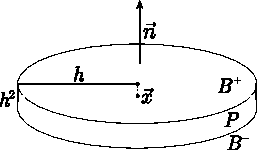
\includegraphics[width=0.6\textwidth]{images/sample.pdf}
%% \caption[caption za v kazalo]{Dolg caption pod sliko}
%  \caption[Primer vektorske slike.]{Primer vektorske slike z oznakami v enaki pisavi, kot jo
%     uporablja \LaTeX{}.  Narejena je s programom Inkscape, \LaTeX{} oznake so importane v
%     Inkscape iz pomožnega PDF.}
%  \label{fig:sample}
%\end{figure}
%
%\begin{figure}[h]
%  \centering
%  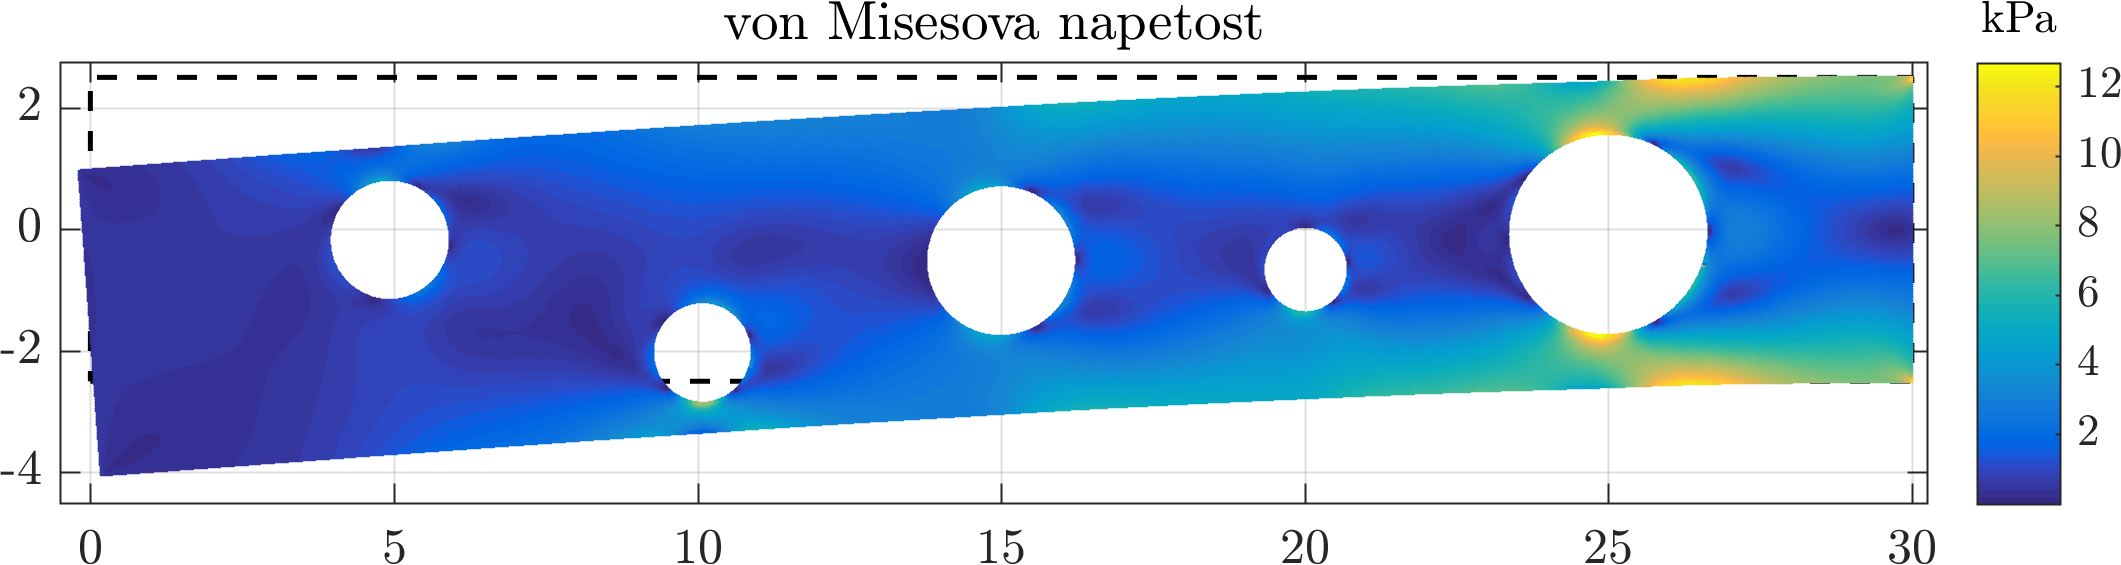
\includegraphics[width=0.8\textwidth]{images/image.png}
%  \caption[Primer bitne slike.]{Primer bitne slike, izvožene iz Matlaba. Poskrbite, da so slike v
%  dovolj visoki resoluciji in da ne vsebujejo prosojnih elementov (to zahteva PDF/A-1b format).}
%  \label{fig:image}
%\end{figure}

%\subsection{Kako narediti stvarno kazalo}
%Dodate ukaze \verb|\index{polje}| na besede, kjer je pojavijo, kot tukaj\index{tukaj}.
%Več o stvarnih kazalih je na voljo na \url{https://en.wikibooks.org/wiki/LaTeX/Indexing}.

%\subsection{Navajanje literature}
%Članke citiramo z uporabo \verb|\cite{label}|, \verb|\cite[text]{label}| ali pa več naenkrat s
%\verb|\cite\{label1, label2}|. Tudi tukaj predhodno besedo in citat povežemo z nedeljivim presledkom
%$\sim$. Na primer~\cite{chen2006meshless,liu2001point}, ali pa \cite{kibriya2007empirical}, ali pa
%\cite[str.\ 12]{trobec2015parallel}, \cite[enačba (2.3)]{pereira2016convergence}.
%Vnosi iz \verb|.bib| datoteke, ki niso citirani, se ne prikažejo v seznamu literature, zato jih
%tukaj citiram.~\cite{vene2000categorical}, \cite{gregoric2017stopniceni}, \cite{slak2015induktivni},
%\cite{nsphere}, \cite{kearsley1975linearly}, \cite{STtemplate}, \cite{NunbergerTand}.

% Literatura:
% Primer navajanja na http://www.fmf.uni-lj.si/storage/24240/LiteraturaM.pdf,
% ampak bi moral stil poskrbeti za vse. Reference se uredijo po abecedi.
% Če nobena izbira izmed @book, @atricle,... ni ok, potem se lahko vse napiše v
% @misc pod note={} in deluje tako kot normalen LaTeX.
% Komentar v bib datoteki se naredi samo s parom { }
% Za urejanje literature avtor priporoča program Jabref, ki zna tudi avtomatsko
% okrajšati imena revij. Za pravilno sortiranje vnosov brez avtorja, uporabite
% polje key={ }, kot v primeru.
% V primeru napak ustvarite issue na GitHubu ali pišite na jure.slak@fmf.uni-lj.si.
\cleardoublepage                           % na desni strani
\phantomsection                            % da prav delujejo hiperlinki
\addcontentsline{toc}{section}{\bibname}   % dodajmo v kazalo
\bibliographystyle{fmf-sl}                 % uporabljen stil je v datoteki fmf-sl.bst, na voljo tudi angleška verzija
\bibliography{\literatura}                 % literatura je v datoteki, definirani na začetku
% TeXStudio zmede \ zgoraj, tako da lahko notri napišeš dejansko ime .bib datoteke, če ti
% ne delajo predlogi citatov.

% Za stvarno kazalo
\cleardoublepage                           % na desni strani
\phantomsection                            % da prav delujejo hiperlinki
\addcontentsline{toc}{section}{\indexname} % dodajmo v kazalo
\printindex

\end{document}
